\chapter{Revue de la Littérature et Concepts de Base sur les méthodes d'ensemble de régression}
\section*{introduction}
Dès \textbf{1997}, le potentiel du \textbf{data mining} pour améliorer les problèmes dans le domaine médical avait été identifié par l'Organisation mondiale de la santé (\textbf{OMS}) (Gulbinat, 1997). L'utilité de la détection de connaissances à partir des dépôts de données médicales a été soulignée par l'OMS, car elle bénéficie au diagnostic médical et à la prédiction. Le data mining est un processus de découverte de connaissances utiles à partir de bases de données pour construire une structure (c'est-à-dire un modèle ou un schéma) qui peut interpréter de manière significative les données. Le data mining est le processus de découverte de schémas et de connaissances intéressants à partir d'une grande quantité de données (Han et al., 2001). Le data mining utilise de nombreuses techniques d'apprentissage automatique pour découvrir des schémas cachés dans les données. Ces techniques peuvent être réparties en trois catégories principales : les techniques d'\textbf{apprentissage supervisé}, les techniques d'\textbf{apprentissage non supervisé} et les techniques d'\textbf{apprentissage semi-supervisé} (Huang al., 2014). Voir figure \ref{fig:machinelearningtype}. Les systèmes experts développés par des techniques d'apprentissage automatique peuvent être utilisés pour aider les médecins dans le \textbf{diagnostic} et la \textbf{prédiction des maladies} (Kononenko, 2001). En raison de l'importance du diagnostic des maladies pour l'humanité, plusieurs études ont été menées sur le développement de méthodes pour leur classification~\cite{Analytical2017Meh}.

\section{Apprentissage Automatique}
Depuis leur évolution, les humains ont utilisé de nombreux types d'outils pour accomplir diverses tâches de manière plus simple. La créativité du cerveau humain a conduit à l'invention de différentes machines. Ces machines ont facilité la vie humaine en permettant aux gens de répondre à divers besoins de la vie, y compris le voyage, les industries et l'informatique. Et l'apprentissage automatique en fait partie. Selon Arthur Samuel, l'\textbf{apprentissage automatique} est défini comme le domaine d'étude qui donne aux ordinateurs la capacité d'apprendre sans être explicitement programmés. \textit{Arthur Samuel} était célèbre pour son programme de jeu de dames. L'apprentissage automatique (\textbf{ML}) est utilisé pour apprendre aux machines comment gérer les données de manière plus efficace. Parfois, après avoir examiné les données, nous ne pouvons pas interpréter les informations extraites des données. Dans ce cas, nous appliquons l'apprentissage automatique. Avec l'abondance des ensembles de données disponibles, la demande pour l'apprentissage automatique est en hausse. De nombreuses industries appliquent l'apprentissage automatique pour extraire des données pertinentes. Le but de l'apprentissage automatique est d'\textit{apprendre à partir des données}~\cite{Machine2020Batta}.
\begin{figure}[!h]
	\centering
	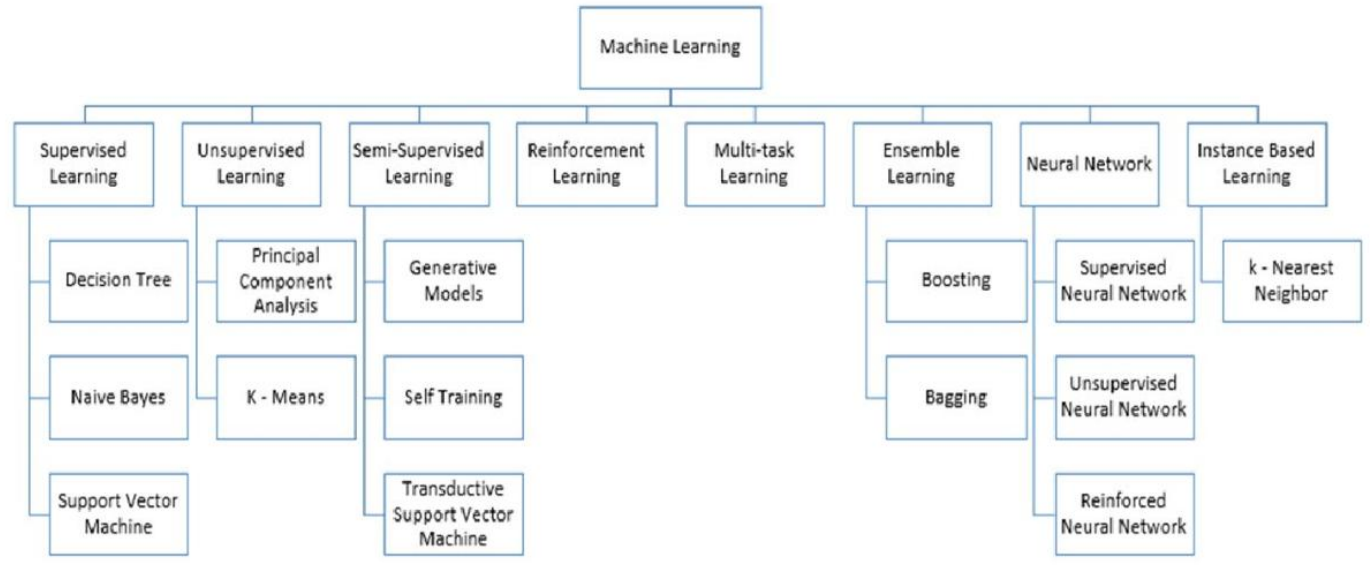
\includegraphics[width=1\linewidth]{images/machineLearningType}
	\caption{Structure arborescente du machine learning ~\cite{mltree}}
	\label{fig:machinelearningtype}
\end{figure}

\subsection{Techniques d'Apprentissage Automatique}
Voici un aperçu rapide de certains des algorithmes couramment utilisés en apprentissage automatique (ML)
\subsubsection{Apprentissage Supervisé}
Les algorithmes d'\textbf{apprentissage supervisé} sont ceux qui nécessitent une assistance externe. L'ensemble de données d'entrée est divisé en ensemble d'entraînement et ensemble de test. L'ensemble d'entraînement a une variable de sortie qui doit être prédite ou classée. Tous les algorithmes apprennent un certain type de schémas à partir de l'ensemble d'entraînement et les appliquent à l'ensemble de test pour la prédiction ou la classification~\cite{Machine2020Batta}. Le flux de travail des algorithmes d'apprentissage supervisé est donné dans la figure \ref{fig:suppervisedlearning} ci-dessous.

Exemple d'apprentissage supervisé :
\begin{itemize}
	\item \textbf{Arbre de Décision} : Algorithme qui construis un modèle arborescent de décisions et de leurs conséquences possibles. Ils divisent les données en fonction des caractéristiques et créent des règles de décision pour la classification ou la régression~\cite{leewayhertzSupervised}. Supposons que vous souhaitiez prédire si un client d'une entreprise de télécommunications va se désabonner ou non. L'algorithme de l'arbre de décision peut utiliser des caractéristiques telles que les données démographiques du client, l'utilisation des services et l'historique des paiements pour créer des règles qui prédisent le désabonnement.
	\item \textbf{Naïve Bayes} : Algorithme probabiliste basé sur le théorème de Bayes et supposant l'indépendance des caractéristiques~\cite{leewayhertzSupervised}. Il est couramment utilisé pour la classification des textes et le filtrage des spams. Par exemple, vous pouvez l'utiliser pour classer les courriels en tant que spam ou ham (non-spam).
\end{itemize}
\begin{figure}[!h]
	\centering
	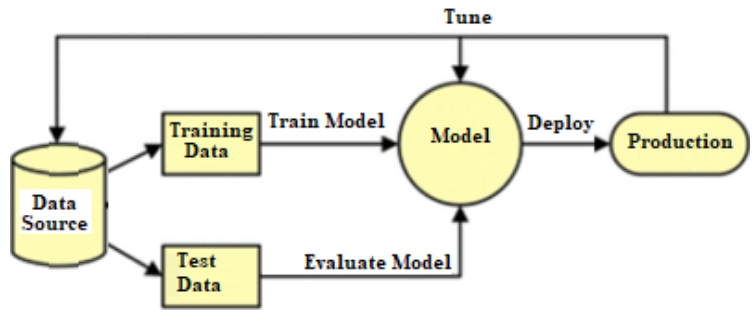
\includegraphics[width=0.9\linewidth]{images/supervisedlearning}
	\caption{Flux de travail de l'apprentissage supervisé~\cite{supervised_learning}}
	\label{fig:suppervisedlearning}
\end{figure}
\newpage
\subsubsection{Apprentissage Non Supervisé}
Contrairement à l'apprentissage supervisé ci-dessus, il n'y a pas de réponses correctes et il n'y a pas de 'professeur'. Les algorithmes sont laissés à leurs propres dispositifs pour découvrir et présenter la structure intéressante dans les données ( Voir la figure \ref{fig:unsupervisedlearning}). Les algorithmes d'apprentissage non supervisé apprennent quelques caractéristiques à partir des données. Lorsque de nouvelles données sont introduites, elles utilisent les caractéristiques apprises précédemment pour reconnaître la classe des données. Il est principalement utilisé pour le \textit{clustering} et la réduction des \textit{features}~\cite{Machine2020Batta}.

\begin{figure}[!h]
	\centering
	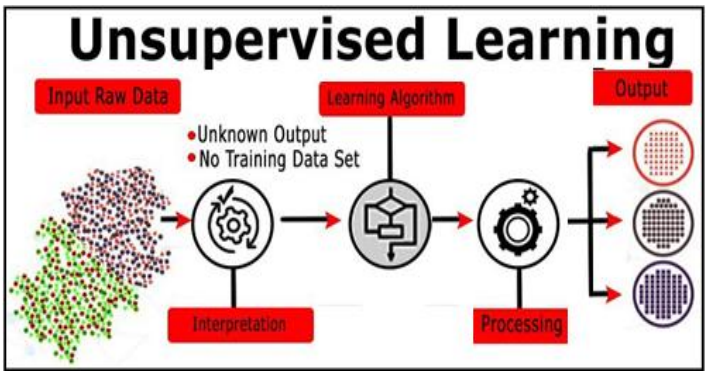
\includegraphics[width=0.8\linewidth]{images/unsupervisedlearning}
	\caption{Schema d'apprentissage Non Supervisé~\cite{lsupervised}}
	\label{fig:unsupervisedlearning}
\end{figure}

Exemple d'apprentissage non supervisé :
\begin{itemize}
	\item \textbf{Clustering K-means} : est l'un des algorithmes d'apprentissage non supervisé les plus simples qui résout le problème bien connu du clustering. La procédure suit une manière simple et facile de classer un ensemble de données donné par un certain nombre de clusters.
\end{itemize}

\subsubsection{Apprentissage Semi-Supervisé}
L'\textbf{apprentissage semi-supervisé} est une combinaison des méthodes d'apprentissage \textit{supervisé} et \textit{non supervisé}. Il peut être fructueux dans les domaines de l'apprentissage automatique et du data mining où les données non étiquetées sont déjà présentes et obtenir les données étiquetées est un processus fastidieux~\cite{Machine2020Batta}. 

\section{Introduction au Deep Learning}

Le \textit{Deep Learning} est une branche de l'intelligence artificielle (IA) qui s'appuie sur des réseaux de neurones artificiels pour modéliser des relations complexes dans les données. Ce domaine a connu une croissance exponentielle grâce aux avancées technologiques en matière de calcul et aux grandes quantités de données disponibles. Ce cours explore les concepts fondamentaux du Deep Learning.

\subsection{Les bases du Deep Learning}

\subsubsection{Réseaux de neurones}
	 Les \textit{neurones artificiels}, inspirés du fonctionnement des neurones biologiques (voir figure \ref{fig:ann}), sont les unités de base des réseaux de neurones. Chaque neurone reçoit des entrées, les traite à l'aide d'une fonction d'activation, puis transmet une sortie.
	 
	 Parmi les caractéristiques nous avons : 
	\begin{itemize}
		\item \textbf{Couches et profondeur} : Les neurones sont organisés en couches (entrée, cachées, sortie). Un réseau est dit "profond" lorsqu'il possède plusieurs couches cachées, permettant ainsi de capturer des abstractions de plus en plus complexes des données d'entrée.
		\item \textbf{Poids et apprentissage} : Chaque connexion entre deux neurones est associée à un poids, qui détermine l'influence de l'entrée sur la sortie. Ces poids sont ajustés lors de la phase d'apprentissage pour minimiser l'erreur du modèle.
	\end{itemize}
	\begin{figure}[h!]
		\centering
		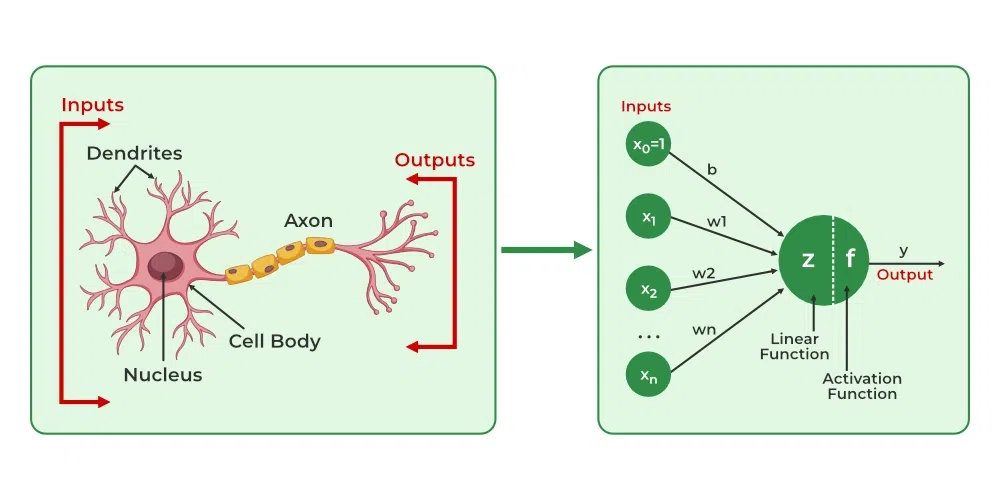
\includegraphics[width=0.9\linewidth]{images/Artificial-Neural-Networks}
		\caption{Neurone Biolique en Artificiel~\cite{geeksforgeeks}}
		\label{fig:ann}
	\end{figure}
	
\subsubsection{Fonctionnement du réseau}
	Le Deep Learning repose souvent sur l'apprentissage supervisé, où le modèle est entraîné à partir d'un ensemble de données étiquetées.
	\begin{itemize}
		\item \textbf{Propagation avant} : Les données d'entrée sont transmises couche par couche, chaque neurone calculant une activation à partir de ses entrées pondérées (Voir figure \ref{fig:backward-propagation})
		\item \textbf{Rétropropagation} : L'algorithme de rétropropagation ajuste les poids en fonction de l'erreur commise par le modèle, en propagant cette erreur en sens inverse, de la sortie vers l'entrée.
	\end{itemize}
	\begin{figure}[h!]
		\centering
		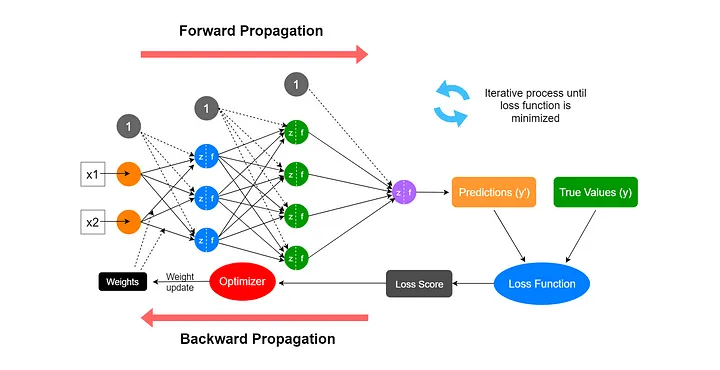
\includegraphics[width=1\linewidth]{images/Backward-Propagation}
		\caption{Fonctionnement réseau de neurone~\cite{fowardpropagation}}
		\label{fig:backward-propagation}
	\end{figure}
	
\subsection{Fonctions d'activation}

Les fonctions d'activation permettent d'introduire de la non-linéarité au sein des réseaux de neurones, ce qui est essentiel pour leur capacité à modéliser des relations complexes entre les variables et à résoudre des problèmes qui ne peuvent être abordés par des modèles linéaires simples.
\subsubsection*{Exemples de fonctions d'activation}

\begin{itemize}
	\item \textbf{ReLU (Rectified Linear Unit)} : 
	\[
	f(x) = \max(0, x)~,
	\]
	où $x$ représente l'entrée d'un neurone. La fonction ReLU renvoie $x$ si celui-ci est positif, sinon elle renvoie $0$. ReLU est couramment utilisée car elle permet un apprentissage efficace tout en réduisant les risques de \textit{vanishing gradient}\footnote{Le \textit{vanishing gradient} est un problème courant dans les réseaux de neurones profonds, où les gradients deviennent extrêmement petits, empêchant les poids des couches précédentes de se mettre à jour correctement, ce qui ralentit considérablement l'apprentissage.}.

	\item \textbf{Sigmoid} : 
	\[
	f(x) = \frac{1}{1 + e^{-x}}~,
	\]
	où $x$ représente l'entrée d'un neurone. la fonction Sigmoid est utilisée pour normaliser la sortie entre 0 et 1, particulièrement utile pour les tâches de classification binaire.
	\item \textbf{Tanh (Tangente hyperbolique)} : 
	\[
	f(x) = \frac{e^x - e^{-x}}{e^x + e^{-x}}~,
	\]
	où $x$ représente l'entrée d'un neurone. Tanh normalise la sortie entre -1 et 1, ce qui peut conduire à une convergence plus rapide que la Sigmoid dans certains cas.
\end{itemize}

\subsection{Entraînement des modèles}

\subsubsection{Fonction de coût}

\begin{itemize}
	\item \textbf{Évaluation de l'erreur} : La fonction de coût mesure l'écart entre les prédictions du modèle et les vraies étiquettes, guidant ainsi l'ajustement des poids.
	\item \textbf{Exemples de fonctions de coût} :
	\begin{itemize}
		\item \textbf{Erreur quadratique moyenne (MSE)} : 
		\[
		\text{MSE} = \frac{1}{n} \sum_{i=1}^{n} (y_i - \hat{y}_i)^2~,
		\]
		où :
		\begin{itemize}
			\item $n$ est le nombre total de points de données,
			\item $y_i$ représente la valeur réelle ou observée pour le $i$-ème point de données,
			\item $\hat{y}_i$ est la valeur prédite par le modèle pour le $i$-ème point de données.
		\end{itemize}
		
		La MSE est une métrique utilisée pour évaluer les modèles de régression. Elle calcule la moyenne des carrés des écarts entre les valeurs réelles et les valeurs prédites. Une MSE plus faible indique que le modèle fait de meilleures prédictions.
		\item \textbf{Erreur quadratique moyenne racine (RMSE)} : 
		\[
		\text{RMSE} = \sqrt{\frac{1}{n} \sum_{i=1}^{n} (y_i - \hat{y}_i)^2}~,
		\]
		où :
		\begin{itemize}
			\item $n$ est le nombre total de points de données,
			\item $y_i$ représente la valeur réelle ou observée pour le $i$-ème point de données,
			\item $\hat{y}_i$ est la valeur prédite par le modèle pour le $i$-ème point de données.
		\end{itemize}
		
		 Le RMSE est une mesure courante de l'erreur dans les problèmes de régression. Il représente la racine carrée de la moyenne des carrés des erreurs entre les valeurs réelles et les valeurs prédites. Contrairement au MSE, le RMSE est dans la même unité que les données, ce qui facilite l'interprétation des résultats. Une valeur de RMSE plus faible indique un meilleur ajustement du modèle aux données.
	
		\item \textbf{R-carré (\( R^2 \))} : 
		\[
		R^2 = 1 - \frac{\sum_{i=1}^{n} (y_i - \hat{y}_i)^2}{\sum_{i=1}^{n} (y_i - \bar{y})^2} ~,
		\]
		où :
		\begin{itemize}
			\item $n$ est le nombre total de points de données,
			\item $y_i$ représente la valeur réelle ou observée pour le $i$-ème point de données,
			\item $\hat{y}_i$ est la valeur prédite par le modèle pour le $i$-ème point de données.
		\end{itemize}
		Le \( R^2 \) score, également appelé \textbf{coefficient de détermination}, mesure la proportion de la variance des données qui est expliquée par le modèle. Un score proche de 1 indique que le modèle explique bien les données, tandis qu'un score proche de 0 indique le contraire.
	\end{itemize}
\end{itemize}

\subsubsection{Optimisation}

L'optimisation est une étape cruciale dans l'entraînement des réseaux de neurones, où l'objectif est de minimiser la fonction de coût en ajustant les poids du réseau. Cela se fait en utilisant des algorithmes d'optimisation qui guident le processus d'ajustement des poids pour réduire l'erreur entre les prédictions du modèle et les valeurs réelles.\\

 \textbf{Descente de gradient} :
	L'algorithme le plus couramment utilisé pour l'optimisation en Deep Learning est la descente de gradient. L'idée principale est de mettre à jour les poids du réseau dans la direction opposée au gradient de la fonction de coût par rapport aux poids. Ce processus est itératif et continue jusqu'à ce que la fonction de coût atteigne un minimum local ou global.
	
	\[
	\theta_{t+1} = \theta_t - \eta \nabla_{\theta} J(\theta_t)~,
	\]
	
	où :
	\begin{itemize}
		\item \( \theta_t \) représente les poids du réseau à l'itération \( t \),
		\item \( \eta \) est le taux d'apprentissage (un hyperparamètre qui contrôle la taille des mises à jour des poids),
		\item \( \nabla_{\theta} J(\theta_t) \) est le gradient de la fonction de coût \( J(\theta) \) par rapport aux poids \( \theta \).
	\end{itemize}

\subsection{Applications du Deep Learning}

\subsubsection*{Vision par ordinateur}

\begin{itemize}
	\item \textbf{Tâches principales} : Classification d'images, détection d'objets, segmentation sémantique.
	\item \textbf{Exemple d'architecture} : Les réseaux de neurones convolutifs (CNN) sont la norme pour les tâches de vision par ordinateur, offrant d'excellentes performances sur des tâches complexes comme la reconnaissance d'images.
\end{itemize}

\subsubsection*{Traitement du langage naturel (NLP)}

\begin{itemize}
	\item \textbf{Tâches principales} : Traduction automatique, résumé de texte, chatbots, analyse de sentiments.
	\item \textbf{Exemple d'architecture} : Les réseaux de neurones récurrents (RNN) et les modèles de transformateurs comme BERT sont souvent utilisés pour comprendre et traiter des textes en capturant les relations entre les mots sur de longues distances dans une phrase ou un document.
\end{itemize}

\section{Ensemble Learning ou Apprentissage par Ensemble}
Le \textit{systèmes d'ensemble}, ont gagné en popularité au sein de la communauté de l'intelligence artificielle et de l'apprentissage automatique au cours des deux dernières décennies. Initialement développés pour réduire la variance et améliorer la précision des décisions automatisées, ces systèmes se sont avérés efficaces et polyvalents dans divers domaines. Ils sont utilisés pour résoudre des problèmes tels que la sélection de caractéristiques, l'estimation de la confiance, et la gestion de données déséquilibrées. Bien que la recherche sur les systèmes d'ensemble soit relativement récente, la prise de décision collective, semblable aux systèmes d'ensemble, fait partie de notre quotidien depuis longtemps, comme en témoignent la démocratie et le système judiciaire~\cite{polikar2012ensemble}.

\subsection{Définition}

L'\textbf{apprentissage par ensemble} est une méthode dans laquelle plusieurs \textbf{modèles} sont créés et combinés de manière stratégique pour améliorer la performance et la robustesse dans la résolution d'un problème spécifique d'intelligence computationnelle\footnote{L'intelligence computationnelle est un domaine qui s'inspire de mécanismes biologiques et cognitifs pour concevoir des systèmes capables de résoudre des problèmes complexes.}. L'apprentissage par ensemble est principalement utilisé pour améliorer les performances d'un modèle ou réduire la probabilité de sélectionner un modèle médiocre~\cite{Machine2020Batta}. 

\subsection{principes de fonctionnement}
Les \textbf{systèmes d'ensemble} sont inspirés par notre pratique quotidienne de consulter divers \textit{experts} avant de prendre des décisions importantes, comme consulter plusieurs médecins avant une opération ou lire des avis avant un achat. Cette approche vise à augmenter notre confiance dans la décision finale en combinant différentes opinions.

En apprentissage automatique, les systèmes d'ensemble améliorent la \textbf{précision} en abordant les deux composantes principales de l'erreur de classification : le \textbf{biais} et la \textbf{variance} (Voir la figure \ref{fig:arr-ens}). Le biais reflète la précision d'un classificateur\footnote{Un classificateur est un modèle d'apprentissage automatique qui affecte une entrée à une catégorie ou classe spécifique en fonction des caractéristiques observées.}, tandis que la variance mesure la précision lors de l'utilisation de différents ensembles de données d'apprentissage. Généralement, un faible biais est associé à une variance élevée, et vice versa. Les systèmes d'ensemble cherchent à créer plusieurs classificateurs avec un biais similaire et à combiner leurs résultats, par exemple par \textbf{moyenne}, pour \textbf{réduire la variance} \cite{polikar2012ensemble}.

\begin{figure}[h!]
	\centering
	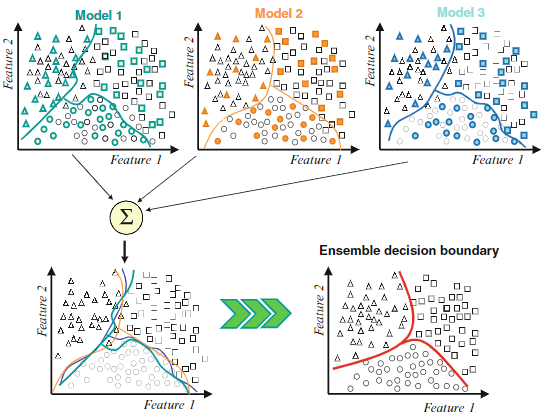
\includegraphics[width=0.8\linewidth]{images/arr-ens}
	\caption{Réduction de la variabilité à l'aide de systèmes d'ensemble\cite{polikar2012ensemble}}
	\label{fig:arr-ens}
\end{figure}
\newpage
\subsection{Techniques d'Ensemble Learning}

Les premiers travaux sur les \textbf{systèmes d'ensemble} sont attribués à Dasarathy et Sheela (1979), qui ont exploré le \textbf{partitionnement de l'espace des caractéristiques} en utilisant plusieurs \textbf{classificateurs}\footnote{Un classificateur est un algorithme d'apprentissage automatique qui attribue une étiquette ou une classe à des données en fonction de leurs caractéristiques observées.}~\cite{dasarathy1979}. Dix ans plus tard, Hansen et Salamon ont démontré que l'utilisation d'un \textbf{système d'ensemble} pouvait améliorer les performances de \textbf{classification}~\cite{hansen1990}. Cependant, c'est Schapire qui a marqué un tournant en introduisant le concept de \textbf{boosting}, montrant qu'un \textbf{classificateur puissant} pouvait être construit à partir de classificateurs ayant une performance légèrement supérieure à celle d'une simple supposition aléatoire~\cite{schapire1990}. Cette théorie a abouti à l'algorithme \textbf{AdaBoost}, largement utilisé pour les problèmes de \textbf{classification multi-classes} et de \textbf{régression}~\cite{freund1997}.

Depuis ces travaux fondateurs, la recherche sur les systèmes d'ensemble s'est intensifiée, donnant naissance à divers algorithmes, chacun ayant des caractéristiques propres : \textbf{bagging}~\cite{breiman1996}, \textbf{RandomForest}, \textbf{MoE}~\cite{jacobs1991}, et \textbf{généralisation par empilement}~\cite{wolpert1992}, entre autres. Ces méthodes se distinguent principalement par la \textbf{sélection des données d'apprentissage}, le mode de \textbf{génération des modèles constitutifs}, et la \textbf{règle de combinaison} employée pour la décision finale, éléments considérés comme les \textbf{piliers} des systèmes d'ensemble.

Ces systèmes sont principalement appliqués dans deux contextes : \textbf{la sélection de classificateurs} et \textbf{la fusion de classificateurs}~\cite{kuncheva2004}. Dans le cadre de la sélection, chaque classificateur est spécialisé dans une région spécifique de l'espace des données, et celui qui correspond le mieux aux données en question est sélectionné pour prendre la décision finale. En revanche, dans la fusion, tous les classificateurs contribuent à la décision, ce qui permet de créer un classificateur composite avec une \textbf{variance} plus faible, réduisant ainsi l'erreur globale~\cite{breiman1996, freund1997}.

\subsubsection*{Construction d'un système d'ensemble}
Trois stratégies doivent être choisies pour construire un système d'ensemble efficace : (1) \textbf{échantillonnage/sélection des données} ; (2) \textbf{formation des classificateurs membres} ; et (3) \textbf{combinaison des classificateurs}.

\subsubsection{Échantillonnage et sélection des données : Diversité}
Dans les \textbf{systèmes d'ensemble}, la diversité des erreurs entre les membres est cruciale. Si tous les membres fournissent les mêmes résultats, leur combinaison n'apporte aucun bénéfice. Il est donc essentiel que les membres commettent des erreurs différentes, idéalement avec des résultats indépendants ou négativement corrélés.

La diversité peut être obtenue par diverses stratégies, comme l'utilisation de différents sous-ensembles des données d'apprentissage. Par exemple, le \textbf{bagging} utilise des répliques bootstrapées des données, tandis que le \textbf{boosting} se concentre sur les échantillons mal classés. D'autres méthodes incluent l'utilisation de sous-ensembles des \textbf{caractéristiques} disponibles ou différents \textbf{classificateurs} de base. Malgré l'importance reconnue de la diversité pour améliorer la performance des ensembles, aucune relation explicite entre la diversité et la précision de l'ensemble n'a été clairement établie ~\cite{polikar2012ensemble}.

\subsubsection{Formation des classificateurs de membres}
Au cœur de tout système basé sur un ensemble se trouve la stratégie utilisée pour former les membres individuels de l'ensemble. De nombreux algorithmes concurrents ont été développés pour former les classificateurs d'ensemble ; cependant, le \textit{bagging} (et les algorithmes apparentés arc-x4 et Random Forest), le \textit{boosting} (et ses nombreuses variations), la \textit{stack generalization} et le \textit{hierarchical MoE} restent les approches les plus couramment employées.

\subsubsection{Combinaison des membres de l'ensemble}
La dernière étape des \textbf{systèmes d'ensemble} est la \textbf{combinaison des classificateurs} individuels. La stratégie de combinaison dépend du type de classificateurs utilisés. Par exemple, certains classificateurs comme les \textbf{Support Vector Machines (SVM)} produisent des sorties discrètes, pour lesquelles les règles de combinaison les plus courantes sont le \textbf{majority voting} (simple ou pondéré) et le \textbf{Borda count}. D'autres classificateurs, tels que le \textbf{multilayer perceptron} ou le \textbf{naïve Bayes classifier}, fournissent des sorties continues indiquant le soutien pour chaque classe. Pour ces classificateurs, une gamme plus large d'options est disponible, telles que les \textbf{arithmetic combinators} (somme, produit, moyenne) ou des \textbf{decision models} plus sophistiqués. Certains de ces combinateurs peuvent être appliqués immédiatement après l'apprentissage, tandis que des méthodes plus complexes comme \textbf{stacking} ou \textbf{hierarchical MoE} peuvent nécessiter une étape d'apprentissage supplémentaire. Nous examinerons brièvement ces approches.
\subsubsection*{Combining Class Labels (Combinaison des étiquettes de classe)}
Cette sous-section se concentre sur les scénarios où les classifieurs produisent des étiquettes de classe discrètes.

\begin{itemize}
	\item \textbf{Majority Voting (Vote majoritaire)} : La classe avec le plus de votes gagne. L'ensemble choisit la classe $\omega_c$, si :
	\[
	\sum_{t=1}^{T} d_{t,c} = \max_{c} \sum_{t=1}^{T} d_{t,c}~,
	\]
	où $d_{t,c}$ est 1 si le classifieur $t$ choisit la classe $c$, et 0 sinon.
	
	\item \textbf{Weighted Majority Voting (Vote majoritaire pondéré)} : Similaire au vote majoritaire, mais le vote de chaque classifieur est pondéré en fonction de ses performances estimées. L'ensemble choisit la classe $c$, si :
	\[
	\sum_{t=1}^{T} w_t d_{t,c} = \max_{c} \sum_{t=1}^{T} w_t d_{t,c}~,
	\]
	où $w_t$ est le poids assigné au classifieur $t$.
	
	\item \textbf{Borda Count (Comptage Borda)} : Les classes sont classées par chaque classifieur, et la classe avec le score cumulé le plus élevé sur tous les classifieurs est sélectionnée.
\end{itemize}

\subsubsection*{Combining Continuous Outputs (Combinaison des sorties continues)}

Cette sous-section traite des cas où les classifieurs produisent des sorties continues, souvent interprétées comme un support ou des probabilités pour chaque classe.

\begin{itemize}
	\item \textbf{Algebraic Combiners (Combinateurs algébriques)} : Les supports pour chaque classe de différents classifieurs sont combinés à l'aide de diverses fonctions mathématiques. Le support total pour la classe $\omega_c$ est représenté comme suit :
	\[
	\mu_c(x) = F [d_{1,c}(x), \ldots, d_{T,C}(x)]~,
	\]
	où $F[]$ peut être la moyenne, la moyenne pondérée, le minimum, le maximum, la médiane, le produit ou la moyenne généralisée.
\end{itemize}
Les méthodes suivantes et leurs formules correspondantes sont :

\begin{itemize}
	\item \textbf{Mean Rule (Règle de la moyenne)} : Le support pour une classe est la moyenne des supports de tous les classifieurs.
	\[
	\mu_c(x) = \frac{1}{T} \sum_{t=1}^{T} d_{t,c}(x)~,
	\]
	
	\item \textbf{Weighted Average (Moyenne pondérée)} : Similaire à la règle de la moyenne, mais le support de chaque classifieur est pondéré.
	\[
	\mu_c(x) = \frac{1}{T} \sum_{t=1}^{T} w_t d_{t,c}(x)~,
	\]
	où $w_t$ est le poids du $t^{\text{ème}}$ classifieur.
	
	\item \textbf{Trimmed Mean (Moyenne tronquée)} : La moyenne est calculée après avoir éliminé un certain pourcentage des supports les plus élevés et les plus bas pour éviter l'influence des valeurs aberrantes.
	
	\item \textbf{Minimum/Maximum/Median Rule (Règle du minimum/maximum/médiane)} : Le support total est le minimum, le maximum ou la médiane des supports de tous les classifieurs.
	
	\item \textbf{Règle du produit} : Le support total est le produit des supports de tous les classifieurs.
	\[
	\mu_c(x) = \frac{1}{T} \prod_{t=1}^{T} d_{t,c}(x)~,
	\]
	où :
	\begin{itemize}
		\item \( \mu_c(x) \) est le support total pour la classe \( c \) donné un exemple \( x \).
		\item \( T \) est le nombre total de classificateurs dans l'ensemble.
		\item \( d_{t,c}(x) \) est la sortie du classificateur \( t \) pour la classe \( c \) concernant l'exemple \( x \).
	\end{itemize}
	
	\item \textbf{Moyenne généralisée} : Une formule générale qui englobe plusieurs des règles ci-dessus comme cas particuliers, en fonction de la valeur du paramètre \( \alpha \).
	\[
	\mu_c(x) = \left( \frac{1}{T} \sum_{t=1}^{T} (d_{t,c}(x))^\alpha \right)^{1/\alpha}~,
	\]
	où :
	\begin{itemize}
		\item \( \alpha \) est un paramètre qui détermine la nature de la moyenne.
	\end{itemize}
	
\end{itemize}
Ces méthodes offrent une gamme d'options pour combiner les sorties de classifieurs individuels dans un ensemble, permettant la flexibilité et l'adaptabilité à différents scénarios de problèmes.

\subsection{Algorithmes populaires basés sur l'ensemble learning}
Une riche collection de classificateurs basés sur des ensembles a été développée au cours des dernières années. Toutefois, nombre d'entre eux sont des variantes des quelques algorithmes bien établis dont les capacités ont également été largement testées et rapportées. Dans cette section, nous présentons une vue d'ensemble de certains des algorithmes d'ensemble les plus importants
\subsubsection{Bagging}
L'algorithme de \textbf{bagging} (Bootstrap Aggregation) de Breiman est une méthode d'\textbf{ensemble learning} simple mais efficace. Il consiste à entraîner plusieurs classificateurs sur différents échantillons \textbf{bootstrapés} du jeu de données d'entraînement. La \textbf{diversité} dans l'ensemble est assurée par les variations dans ces échantillons et l'utilisation de \textbf{classificateurs faibles} comme les \textit{decision stumps} ou les \textit{SVM linéaires}. La décision finale est prise par un \textbf{vote majoritaire}. Le \textbf{bagging} est particulièrement utile pour les petits jeux de données d'entraînement, tandis qu'une variante appelée \textit{Pasting Small Votes} traite les grands jeux de données en les partitionnant en segments plus petits. L'algorithme de \textbf{Random Forest} est une extension notable du \textbf{bagging}, combinant des \textbf{arbres de décision} entraînés avec une sélection aléatoire des instances et des caractéristiques~\cite{polikar2012ensemble}.
%\begin{algorithm}
%	\caption{An algorithm with caption}\label{alg:cap}
%	\begin{algorithmic}
%		\Require $n \geq 0$
%		\Ensure $y = x^n$
%		\State $y \gets 1$
%		\State $X \gets x$
%		\State $N \gets n$
%		\While{$N \neq 0$}
%		\If{$N$ is even}
%		\State $X \gets X \times X$
%		\State $N \gets \frac{N}{2}$  \Comment{This is a comment}
%		\ElsIf{$N$ is odd}
%		\State $y \gets y \times X$
%		\State $N \gets N - 1$
%		\EndIf
%		\EndWhile
%	\end{algorithmic}
%\end{algorithm}

\begin{algorithm}
	\caption{Bagging~\cite{polikar2012ensemble}}
	\textbf{Entrées :} Données d'entraînement $S$ ; algorithme d'apprentissage supervisé \textit{BaseClassifier} ; entier $T$ spécifiant la taille de l'ensemble ; pourcentage $R$ pour créer les données d'entraînement bootstrapées.
	\begin{algorithmic}
		\For{$t = 1, \dots, T$}
		\State Prendre une réplique bootstrapée $S_t$ en sélectionnant aléatoirement $R\%$ de $S$.
		\State Appeler \textit{BaseClassifier} avec $S_t$ et recevoir l'hypothèse (classifieur) $h_t$.
		\State Ajouter $h_t$ à l'ensemble, $\mathcal{H} = \mathcal{H} \cup \{h_t\}$.
		\EndFor\\\\
		\textbf{Combinaison de l'ensemble : Vote majoritaire simple}\\
		\State Étant donné une instance non étiquetée $x$ :
		\For{$t = 1, \dots, T$}
		\State Évaluer l'ensemble $\mathcal{H} = \{h_1, \dots, h_T\}$ sur $x$.
		\State Laisser $v_{t,c} = 1$ si $h_t$ choisit la classe $\omega_c$, et 0 sinon.
		\EndFor
		\State Obtenir le total des votes reçus par chaque classe : $V_c = \sum_{t=1}^{T} v_{t,c}, \; c = 1, \dots, C$.
		\State \textbf{Sortie :} Classe avec le plus grand $V_c$.
	\end{algorithmic}
\end{algorithm}


\subsubsection{Boosting et AdaBoost}
\textbf{Boosting}, introduit dans le travail \textit{séminal de Schapire} sur le renforcement de l'apprentissage faible, est une approche itérative pour générer un classifieur fort, capable d'atteindre une erreur d'apprentissage arbitrairement faible, à partir d'un ensemble de classifieurs faibles, chacun étant à peine meilleur qu'un choix aléatoire. Bien que le \textbf{Boosting} combine également un ensemble de classifieurs faibles en utilisant un \textbf{vote majoritaire simple}, il diffère du \textbf{Bagging} sur un point crucial. Dans le \textbf{Bagging}, les instances sélectionnées pour entraîner des classifieurs individuels sont des répliques bootstrapées des données d'entraînement, ce qui signifie que chaque instance a une chance égale d'être dans chaque ensemble de données d'entraînement. En revanche, dans le \textbf{Boosting}, l'ensemble de données d'entraînement pour chaque classifieur suivant se concentre de plus en plus sur les instances mal classées par les classifieurs générés précédemment.

Le \textbf{Boosting}, conçu pour des problèmes de classification binaire, crée des ensembles de trois classifieurs faibles à la fois : le premier classifieur (ou hypothèse) $h_1$ est entraîné sur un sous-ensemble aléatoire des données d'entraînement disponibles, similaire au \textbf{Bagging}. Le deuxième classifieur, $h_2$, est entraîné sur un autre sous-ensemble des données d'origine, dont précisément la moitié est correctement identifiée par $h_1$ et l'autre moitié est mal classée. Un tel sous-ensemble d'entraînement est considéré comme le "plus informatif", étant donné la décision de $h_1$. Le troisième classifieur $h_3$ est ensuite entraîné avec les instances sur lesquelles $h_1$ et $h_2$ ne sont pas d'accord. Ces trois classifieurs sont ensuite combinés par un vote majoritaire à trois voies. Schapire a prouvé que l'erreur d'apprentissage de cet ensemble de trois classifieurs est bornée par $g(\epsilon) < 3\epsilon^2 - 2\epsilon^3$, où $\epsilon$ est l'erreur de chacun des trois classifieurs, à condition que chaque classifieur ait un taux d'erreur $\epsilon < 0.5$, ce qui est le minimum attendu d'un classifieur dans un problème de classification binaire.

\textbf{AdaBoost} (pour \textit{Adaptive Boosting}) et ses nombreuses variations ont ensuite étendu l'algorithme original de \textbf{Boosting} à des problèmes de classification multiple (\textbf{AdaBoost.M1}, \textbf{AdaBoost.M2}), ainsi qu'à des problèmes de régression (\textbf{AdaBoost.R}). Ici, nous décrivons l'\textbf{AdaBoost.M1}, la version la plus populaire des algorithmes \textbf{AdaBoost}.

L'\textbf{AdaBoost} présente deux différences fondamentales par rapport au \textbf{Boosting} : (1) les instances sont sélectionnées dans les ensembles de données successifs à partir d'une distribution d'échantillons itérativement mise à jour des données d'entraînement ; et (2) les classifieurs sont combinés par un \textbf{vote majoritaire pondéré}, où les poids des votes sont basés sur les erreurs d'entraînement des classifieurs, elles-mêmes pondérées selon la distribution d'échantillons. La distribution d'échantillons garantit que les échantillons plus difficiles, c'est-à-dire les instances mal classées par le classifieur précédent, sont plus susceptibles d'être inclus dans les données d'entraînement du classifieur suivant.

Dans le pseudocode de l'\textbf{AdaBoost.M1} . La distribution d'échantillons, $D_t(i)$, attribue essentiellement un poids à chaque instance d'entraînement $x_i$, $i = 1, \dots, N$, à partir de laquelle les sous-ensembles de données d'entraînement $S_t$ sont tirés pour chaque classifieur consécutif (hypothèse) $h_t$. La distribution est initialisée pour être uniforme ; ainsi, toutes les instances ont la même probabilité d'être incluses dans le premier ensemble de données d'entraînement. L'erreur d'entraînement $\epsilon_t$ du classifieur $h_t$ est ensuite calculée comme la somme des poids de distribution de ces instances mal classées par $h_t$. L'\textbf{AdaBoost.M1} exige que cette erreur soit inférieure à $1/2$, laquelle est ensuite normalisée pour obtenir $\beta_t$, tel que $0 < \beta_t < 1$ pour $0 < \epsilon_t < 1/2$~\cite{polikar2012ensemble}.
\subsection*{Exemples de Modèles Utilisant Boosting ou AdaBoost}

\begin{itemize}
	\item \textbf{AdaBoost (Adaptive Boosting)} : 
	AdaBoost est l'un des premiers algorithmes de boosting. Il combine plusieurs classificateurs faibles, souvent des arbres de décision simples appelés ``stumps'', pour former un classificateur fort.
	\item \textbf{Gradient Boosting Machine (GBM)} : 
	Cet algorithme construit des modèles de manière séquentielle, en ajustant les erreurs résiduelles de chaque itération précédente. Chaque nouveau modèle corrige les erreurs du modèle précédent.
	
	\item \textbf{XGBoost (Extreme Gradient Boosting)} : 
	XGBoost est une version optimisée de l'algorithme de gradient boosting. Il est réputé pour sa rapidité et son efficacité, particulièrement sur de grandes bases de données. Il est largement utilisé dans les compétitions \texttt{Kaggle} pour des tâches de classification et de régression.
	
	\item \textbf{LightGBM} : 
	LightGBM est une implémentation de boosting conçue pour être plus rapide et plus économe en mémoire que XGBoost, tout en offrant une haute performance. Il est couramment utilisé pour des problèmes de classification et de régression.
	
	\item \textbf{CatBoost} : 
	CatBoost est un algorithme de boosting développé par Yandex, qui est particulièrement efficace pour traiter automatiquement les variables catégorielles. Il est utilisé dans divers contextes de classification et de régression.
\end{itemize}
\begin{algorithm}
	\caption{AdaBoost.M1~\cite{polikar2012ensemble}}
	\textbf{Entrées :} Données d'apprentissage $\mathcal{D} = \{(x_i, y_i)\}$, $i = 1, \dots, N$, $y_i \in \{\omega_1, \dots, \omega_C\}$, apprenant supervisé \textit{BaseClassifier}; taille de l'ensemble $T$. \\
	\textbf{Initialiser :} $D_1(i) = \frac{1}{N}, \forall i = 1, \dots, N$ \\
	\textbf{Pour} $t = 1, 2, \dots, T$ \textbf{faire} : \\
	\begin{algorithmic}[1]
		\State Tirer un sous-ensemble d'apprentissage $S_t$ à partir de la distribution $D_t$.
		\State Entraîner \textit{BaseClassifier} sur $S_t$, recevoir l'hypothèse $h_t: X \rightarrow Y$.
		\State Calculer l'erreur de $h_t$ :
		\[
		\epsilon_t = \sum_{i=1}^{N} \mathbf{I}[h_t(x_i) \neq y_i] \cdot D_t(i)
		\]
		\If{$\epsilon_t > \frac{1}{2}$}
		\State \textbf{abandonner}.
		\EndIf
		\State Définir 
		\[
		\beta_t = \frac{\epsilon_t}{1 - \epsilon_t}
		\]
		\State Mettre à jour la distribution d'échantillonnage :
		\[
		D_{t+1}(i) = \frac{D_t(i)}{Z_t} \times 
		\begin{cases}
			\beta_t, & \text{si } h_t(x_i) = y_i \\
			1, & \text{sinon}
		\end{cases}
		\]
		où $Z_t = \sum_{i=1}^{N} D_t(i)$ est une constante de normalisation pour garantir que $D_{t+1}$ est une fonction de distribution appropriée.
		
		\State \textbf{Vote majoritaire pondéré :} Étant donné une instance non étiquetée $z$, obtenir le total des votes reçus par chaque classe :
		\[
		V_c = \sum_{t: h_t(z)=\omega_c} \log \frac{1}{\beta_t}, \quad c = 1, \dots, C
		\]
		\textbf{Sortie :} Classe avec le plus grand $V_c$.
	\end{algorithmic}
\end{algorithm}
\newpage
\subsection{Tableau comparative entre le Bagging et le Boosting}
Le tableau \ref{tab:bagging_vs_boosting} fait une comparaison sur certains critères entre le Bagging et Boosting
\begin{table}[h!]
	\centering
	\caption{Comparaison entre Bagging et Boosting}
	\begin{tabular}{|p{0.2\textwidth}|p{0.4\textwidth}|p{0.4\textwidth}|}
		\hline
		\textbf{Critère} & \textbf{Bagging} & \textbf{Boosting} \\
		\hline
		\textbf{Principe} & Méthode simple de combinaison des prédictions appartenant au même type. & Méthode de combinaison des prédictions appartenant à des types différents. \\
		\hline
		\textbf{Objectif} & Vise à diminuer la variance, mais pas le biais. & Vise à diminuer le biais, mais pas la variance. \\
		\hline
		\textbf{Poids des Modèles} & Chaque modèle reçoit un poids égal. & Les modèles sont pondérés en fonction de leur performance. \\
		\hline
		\textbf{Indépendance des Modèles} & Chaque modèle est construit indépendamment. & Les nouveaux modèles sont influencés par la performance des modèles précédents. \\
		\hline
		\textbf{Sélection des Données} & Différents sous-ensembles de données d'entraînement sont sélectionnés par échantillonnage aléatoire avec remplacement et méthodes d'échantillonnage aléatoire à partir de l'ensemble des données d'entraînement. & Les modèles sont entraînés de manière itérative, chaque nouveau modèle se concentrant sur la correction des erreurs (mauvais classifications ou résidus élevés) des modèles précédents. \\
		\hline
		\textbf{Problèmes Abordés} & Bagging essaie de résoudre le problème du surajustement (overfitting). & Boosting essaie de réduire le biais. \\
		\hline
		\textbf{Classification des Modèles} & Dans Bagging, les classificateurs de base sont entraînés en parallèle. & Dans Boosting, les classificateurs de base sont entraînés de manière séquentielle. \\
		\hline
		\textbf{Exemples} & Le modèle Random Forest utilise Bagging. & AdaBoost,XGBooost utilisent des techniques de Boosting. \\
		\hline
	\end{tabular}
	\label{tab:bagging_vs_boosting}
\end{table}

Parmi les travaux internationaux sur le chikungunya en utilisant l'ensemble learning nous avons : 

 \textit{Data Science System of Predicting and Detecting the Chikungunya Virus using Ensemble Techniques} par \textbf{Bommireddy Vijay Kumar Reddy, Shail Patel, Anayna Singh } et \textbf{al} le \textit{29 Decembre 2022} : . L'objectif principal des auteurs est d'utiliser des techniques d'ensemble pour trouver une approche novatrice et comparer ces techniques d'ensemble.
 
